\section{Introduktion}

Til diagnosticering af patienter med visse former for sygdomme i hjerneregionen, fortages der ofte scanninger vha. Positron Emission Tomography (PET). 

PET scannere fungerer ved, at man injicerer et radioaktivt sporstof
ind i et legeme. Dette sporstof flyder ud i blodet og bliver bundet
der, hvor der benyttes mest energi, for eksempel en kræftcelle i
hjernen. Dette udsender stråling, som PET scanneren kan opfange.
Strålingsaktiviteten måles for at finde ud af hvor i legemet, der er
mest aktivitet.

PET har dog visse problemer. Man fanger kun strålingskoncentration,
så det er umuligt at se knogle, luft eller blødt væv. Dette giver
problemer, da forskelligt væv afbøjer fotoner i forskellige grad,
og luft næsten ikke gør, forårsager det forringelser i kvaliteten
af scanningen, da man ikke er sikker på, hvad fotonerne har bevæget
sig igennem og dermed, hvor meget de er blevet afbøjet. Hvis man ikke
kender dette, kan man ikke med sikkerhed bestemme deres oprindelsessted.
Dette betragtes, som den væsentligste årsag til forringelse af
billederne~\cite{vigtighedAfAttenuation}. At udbedre denne forringelse er
attenuationskorrigering.

For at udbedre denne forringelse har man kombineret Computed
Tomo\-graphy- (CT) og PET scannere. CT er et røntgenstrålingscan,
der registrerer placering af knogle. Denne information kan man bruge
til at attenuationskorrigere og dermed få et mere korrekt resultat.
CT har dog andre problemer, da den ikke indeholder information om de
bløde vævstyper i hjernen, og derfor ikke er interessant i sig selv, når
man diagnosticerer hjernen. Derudover har røntgenstråling også
en væsentligt risiko for at forårsage yderlig skade~\cite{skadeligCT}.

For at måle det bløde væv kan Magnetic Resonance(MR) benyttes.
MR magnetiserer et legeme svagt, når dette stoppes vil legemet hurtigt
gendanne sit normalt magnetfelt. Hastigheden med hvilken den gendannes
afhænger af vævet. MR scanneren varierer magnetiseringen og starter og
stopper det gentagne gange for at kortlægge legemet. Dette giver billeder
af hjernevæv i høj kvalitet.

Som med CT er MR også blevet sammensat med PET til en PET/MR scanner,
men den kan ikke bruges til attenuationskorrigering, da knogle og luft
begge gendanner deres magnetfelt så hurtigt, at det er meget svært at
måle forskel. Effekten er at knoglen kommer til at ligne luft på
billederne. Dette problem er forsøgt løst på flere måde.

På Rigshospitalet har man hidtil kombineret MR billeder med CT billeder
for at kunne lave attenuationskorrigerede $\mu$-maps kaldet FullCT.
Dette medfører dog det tidligere nævnte problem med den skadende
effekt af røntgenstråling, og man skal flytte patienten rundt mellem
flere scannere. Da scanningerne er foretaget på forskellige scannere,
kan man ikke forvente at patienterne ligger ens. Dette problem skal
også løses. Derfor er man særdeles interesserede i at foretage
attenuationskorrigering alene vha. MR.

Der er to hovedretninger til at udregne CT data ud fra MR data. De
anatomiske og de voxelbaserede. De anatomiske forsøger at kortlægge
hjernen og beskrive generelle træk, de matcher patientdata op imod
et udregnet atlas, og forsøger at korrigere ud fra det~\cite{atlas1,
atlas2}. Det giver nogle problemer ved atypisk anatomi, men har vist sig
at producere gode resultater.

Alternativt er der voxelbaserede metoder, som for hvert voxel forsøger
at bestemme, hvilken type væv den tilhører, men her er det selvfølgelig
virkelig et problem, at man ikke kan skelne mellem luft og knogle.

Ved at benytte meget korte ekko-sekvenser, kaldet UTE (Ultrashort Echo
Times), er det muligt at registrere knogle på MR-scannere. Man måler fra
to forskellige vinkler og med to forskellige echo tider. Der hvor der er
sket en markant ændring i mellem de to billeder, kan da formodes at være
knogle. Implementationen af dette på Siemens scannerne, som Rigshospitalet
benytter, har dog vist sig ikke at være på højde med kombinationen af
CT og MR billeder.

\begin{figure}
    \centering
    \begin{subfigure}{0.3\textwidth}
        \centering
        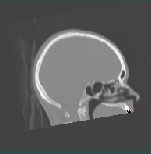
\includegraphics[width=0.75\textwidth]{billeder/ct.png}
        \caption{CT.}
        \label{eksempel:ct}
    \end{subfigure}\hfill
    \begin{subfigure}{0.3\textwidth}
        \centering
        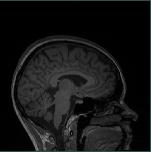
\includegraphics[width=0.75\textwidth]{billeder/mr.png}
        \caption{MR.}
        \label{eksempel:mr}
    \end{subfigure}\hfill
    \begin{subfigure}{0.3\textwidth}
        \centering
        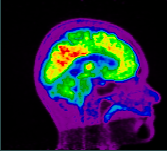
\includegraphics[width=0.75\textwidth]{billeder/pet.png}
        \caption{PET.}
        \label{eksempel:pet}
    \end{subfigure}\hfill
    \caption{Eksempler på billeder. Bemærk at de kun er en slice af et 3D billede.}
    \label{eksempel}
\end{figure}


Målet med denne opgave er at implementere metoden beskrevet i
Johansson et al.~\cite{johansson}, som kan udregne et substitut-CT (sCT)
ud fra fire UTE sekvenser og et T2-vægtet MR billede for en vilkårlig
patient. Dette vil vi gøre ved at træne en Gaussian Mixture Regression
model ud fra disse serier samt et CT målt på samme patient.

Det forventes at læseren kender til basale metoder og termer inden for
billedbehandling og maskinlæring.
